%ju 31-Dez-22 02-Sensoren-und-Aktoren.tex
\textbf{Sensoren} erfassen physikalische Effekte (Druck, Temperatur) und
wandeln diese in elektrische Signale um. (Sinne des Autos)

\textbf{Aktoren} wandeln elektrische Spannungssignale in physikalische
Effekte um (Stellglieder, Ausführen).

\section{Pulsweitenmodulation}\label{pulsweitenmodulation}

\begin{enumerate}
\item
  \textbf{PWM-Signal:} Rechtecksignal (vgl. Kennlinie)
\item
  \textbf{Messen:} Oszilloskop
\item
  \textbf{Ansteuerung:} $0 - 100~\%$, Impuls-Pause-Verhältnisänderung
  (nur Pulsweite ändert sich), aber Periodendauer / Frequenz bleibt
  konstant (keine Spannungsänderung!)
\item
  \textbf{Anwendung}

  \begin{itemize}
  \item
    Elektromotor (Drehzahl)
  \item
    Glühlampen (Helligkeit, dimmen)
  \item
    Beleuchtung, Beispiel: Einfaden-Glühlampe (Standlicht + Bremslicht)
  \end{itemize}
\end{enumerate}

Die \textbf{Pulsweitenmodulation} (PWM) ist eine digitale
Modulationsart, bei der eine technische Größe zwischen zwei Werten
(Spannungspegel $0~V$ und VCC) wechselt. Dabei wird bei konstanter
Frequenz ein Rechtecksignal moduliert, das in Pulsweite (\emph{oder}
Breite bzw. Länge) variiert. Das Verhältnis zwischen Impuls und Pause
(Ein- und Ausschaltzeit) wird als \textbf{Tastgrad / Tastverhältnis}
bezeichnet. \textbf{Anwendung} in der Steuer- und Regelungstechnik.

\section{Halbleiter}\label{halbleiter}

\textbf{Halbleiter} ist ein kristalliner Stoff, der sich bei tiefen
Temperaturen wie ein Isolator verhält und bei höheren Temperaturen nimmt
die elektrische Leitfähigkeit zu. Der Widerstand ist temperaturabhängig.

\textbf{Halbleiterwerkstoffe}

\begin{itemize}
\item
  \textbf{Metalle} Beispiel: Eisen, Kupfer
\item
  \textbf{Isolierstoffe} Beispiel: Kunststoff
\item
  \textbf{Halbleitermaterial} Beispiel: reines Silizium / Germanium
  \textbf{Anwendung} Beispiel: Diode, Transistor
\end{itemize}

\textbf{Dotieren} reines Silizium / Germanium wird verunreinigt, um die
elektrische Leitfähigkeit zu verbessern.

\textbf{P-Leiter und N-Leiter}

\begin{figure}[!ht]% hier: !ht
\centering
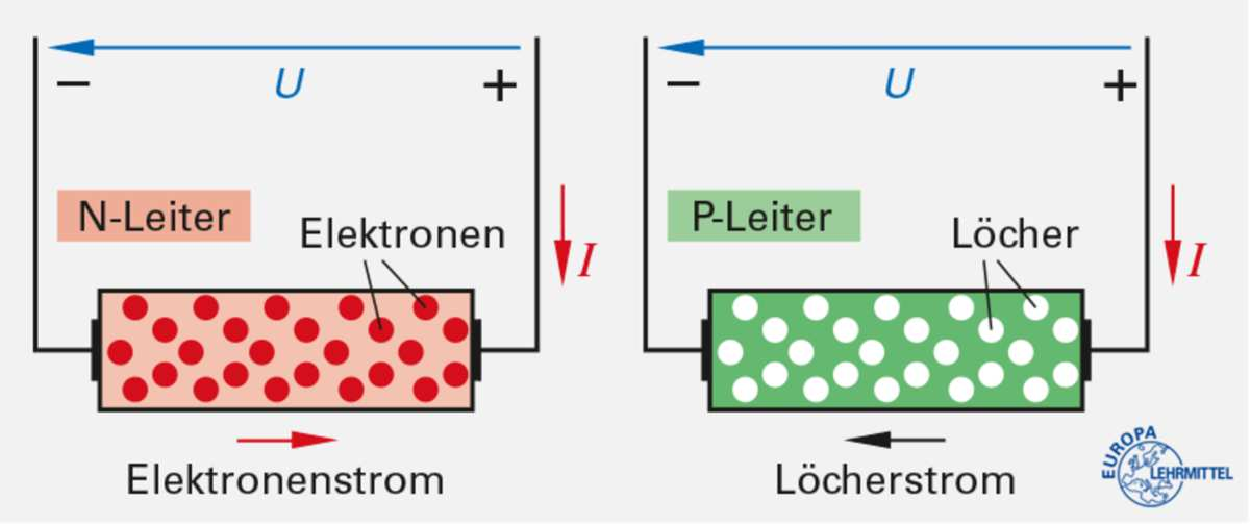
\includegraphics[width=0.4\textwidth]{images/Sensoren/Sensoren-1.pdf}
\caption{Elektronenstrom und Löcherstrom, Quelle: Europa-Verlag}
%\label{fig:}%% anpassen
\end{figure}

\begin{enumerate}
\item
  \textbf{P-Leiter} entsteht, wenn das Leitermaterial Silizium
  verunreinigt wird mit Bohr und bei \emph{Elektronenmangel} enthält es
  freie positive Ladungen. Löcherstrom
\item
  \textbf{N-Leiter} entsteht, wenn das Leitermaterial Silizium
  verunreinigt wird mit Phosphor und bei \emph{Elektronenüberschuss}
  enthält es freie negative Ladungen. Elektronenstrom
\end{enumerate}

$\to$ Legt man an den Halbleiterkristall eine elektrische Spannung an,
dann kommt es zum Elektronenfluss, weil die Elektronen versuchen sich
auszugleichen.

\section{Halbleiterwiderstände NTC und
PTC}\label{halbleiterwiderstaende-ntc-und-ptc}

\begin{figure}[!ht]% hier: !ht
\centering
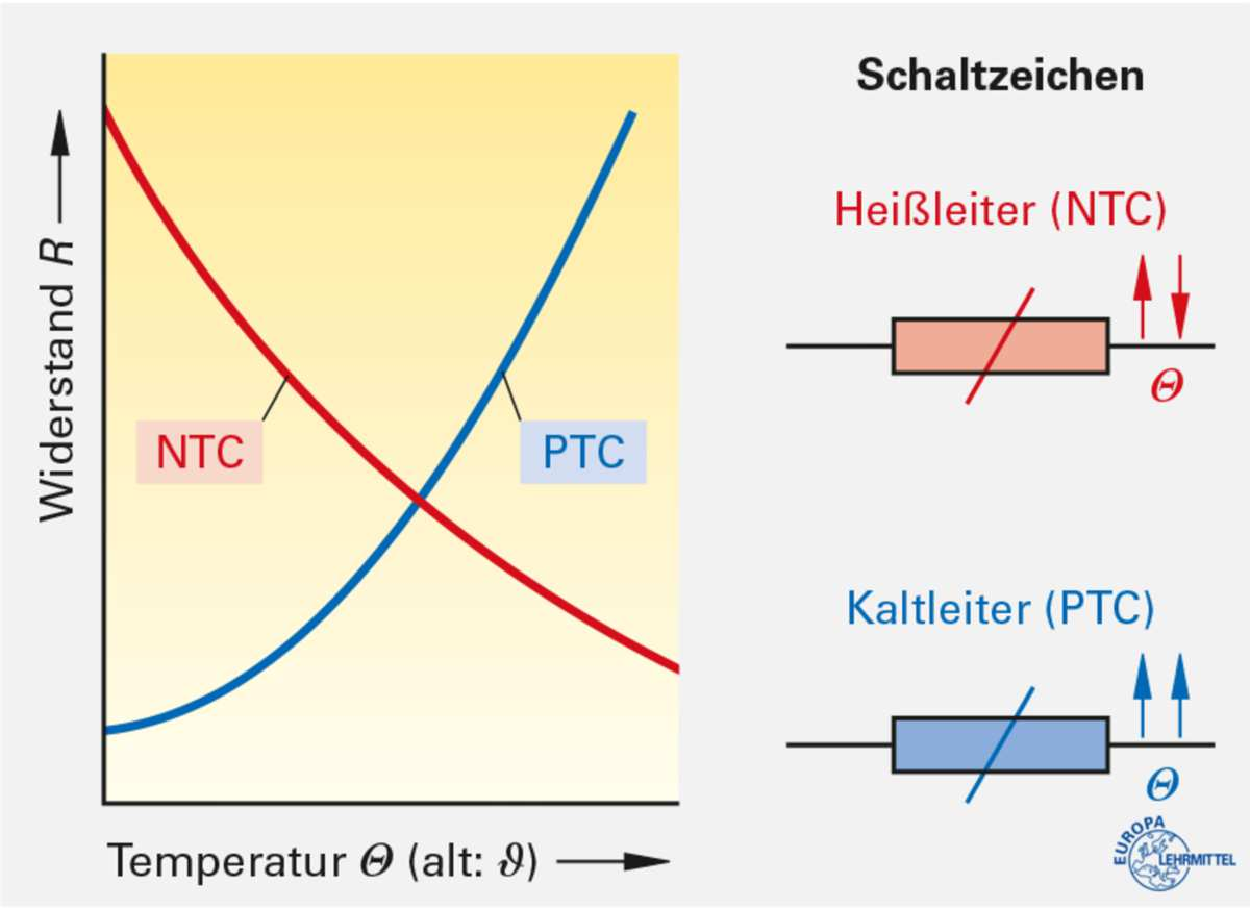
\includegraphics[width=0.4\textwidth]{images/Sensoren/Sensoren-2.pdf}
\caption{NTC und PTC, Quelle: Europa-Verlag}
%\label{fig:}%% anpassen
\end{figure}

\begin{enumerate}
\item
  \textbf{Heißleiter} $\to$ NTC-Widerstände bis $250^\circ\text{C}$

  \begin{itemize}
  \item
    \emph{negativer Temperatur-Koeffizient} $\to$ fallender Widerstand
    bei steigender Temperatur $\uparrow \downarrow$
  \item
    vgl. Kennlinie (x = Temperatur, y = Widerstand)
  \item
    \textbf{Anwendung:} Temperatursensoren (Kühlmittel-, Kraftstoff-,
    Luft-, Motortemperaturfühler)
  \item
    typische Werte: Kalt: $2 - 4~k\Omega$ und Warm:
    $200 - 400~\Omega$
  \item
    \emph{Leitfähigkeit} steigt mit zunehmender Temperatur
  \item
    Widerstand und Spannungsfall am NTC werden kleiner
  \end{itemize}
\item
  \textbf{Kaltleiter} $\to$ PTC-Widerstände bis
  $950 - 1000^\circ\text{C}$

  \begin{itemize}
  \item
    \emph{positiver Temperatur-Koeffizient} $\to$ zunehmender
    Widerstand bei steigender Temperatur $\uparrow \uparrow$
  \item
    vgl. Kennlinie (x = Temperatur, y = Widerstand)
  \item
    \textbf{Anwendung:} Hochtemperaturbereich
    (Diesel-Abgastemperatursensoren), Glühkerzen, Heizungen von
    Lambdasonden
  \item
    \emph{Leitfähigkeit} verringert sich mit zunehmender Temperatur
  \item
    Widerstand und Spannungsfall am PTC werden größer
  \item
    >>Je höher der Widerstand, desto geringer der Stromfluss.<<
  \end{itemize}
\end{enumerate}
